\documentclass[a4paper,14pt]{extarticle} %размер бумаги устанавливаем А4, шрифт 14пунктов
\usepackage[left=2cm,right=2cm,top=2cm,bottom=2cm,bindingoffset=0cm]{geometry} % Меняем поля страницы
\usepackage{setspace}
\onehalfspacing % Полуторный интервал

\usepackage[T2A]{fontenc}
\usepackage[utf8]{inputenc}

\usepackage[english,russian]{babel} %используем русский и английский языки с переносами
\usepackage{amssymb,amsfonts,amsmath,mathtext,cite,enumerate,float} %подключаем нужные пакеты расширений

\usepackage[pdftex]{graphicx, color}
\usepackage{subfigure}
\usepackage{color}
\usepackage{listings}

\usepackage{algorithm}
\usepackage{algpseudocode}

\usepackage{pdflscape}

\usepackage{longtable}

\usepackage{float}
\floatname{algorithm}{Листинг}

\DeclareGraphicsExtensions{.png,.pdf,.jpg,.mps,.bmp}
\graphicspath{{pictures/}} %путь к рисункам
\usepackage{bmpsize}

\usepackage[nooneline]{caption} \captionsetup[table]{justification=raggedleft} \captionsetup[figure]{justification=centering,labelsep=endash}

\begin{document} 
\renewcommand{\figurename}{Рисунок}
\renewcommand{\baselinestretch}{1.5}
\renewcommand{\abstractname}{{Аннотация}}

\renewcommand{\contentsname}{\centering Разделы}
\tableofcontents
\newpage

\iffalse
\section{Общие положения}
\hspace{\parindent} В дипломной работе рассматривается задача распознавания модели автомобиля по фотографии и, хотя на данный момент уже существуют решения в данной области, до сих пор остается не изученной проблема дообучения таких систем. Базовый подход заключается в применении методов машинного обучения (ML --- Machine Learning), таких как нейронные сети (NN --- Neural Network, или ANN --- Artificial Neural Network) и деревья принятия решений (decision tree).

\section{Машинное обучение}
\hspace{\parindent} Машинное обучение можно определить как математическую дисциплину, или набор математических, статистических, численных методов и различных подходов из теории вероятностей для решения задачи автоматического выделения информации (information extraction) и ее интеллектуального анализа (data mining) из неструктурированного набора входных данных. Более подробно --- ставится задача сопоставления заданному значению (объекту) некоторого действия (ответа), таким образом можно говорить об обобщении задачи аппроксимации функции. 

Машинное обучение активно используется при классификации данных, например, распределение новостных статей по рубрикам. Отдельное внимание уделяется обработке изображений, их автоматическому аннотированию~\cite{farabet2013learning} или выделению одного определенного объекта на изображении,  задача распознавания рукописного текста (OCR --- Optical Character Recognition).

Основные подходы машинного обучения при работе с изображениями --- это использование нейронных сетей и деревьев принятия решений. Оба метода занимаются выделением опорных признаков на обрабатываемой картинке, после чего по ним выполняют классификацию. Перед использованием построенной модели ее необходимо обучить на тестовом наборе данных, выработать базу признаков. Алгоритмы обучения решают задачу оптимизации, занимаются подбором неизвестных коэффициентов в математической модели описывающей конкретный метод машинного обучения. Процесс обучения требует большого количества вычислительных операций, что заставляет искать альтернативные подходы при работе с предметной областью, в которую могут добавляться новые классы объектов. Вместо полного переобучения модели используют алгоритмы частичной корректировки коэффициентов (fine tuning). Такой подход дообучения требует меньше времени, но связан с потерей качества, так как не добавляет в модель признаков объектов новых классов.
\fi

\section{Деревья принятия решений} 
\hspace{\parindent} Дерево принятия решений является графом, в узлах которого записаны условия определяющие переход в следующую вершину, а в листьях хранятся значения целевой функции (рисунок~\ref{fig:decision-tree}). Таким образом, решение задачи сводится к спуску из корня дерева до его листа.

\begin{figure}[H]
\centering
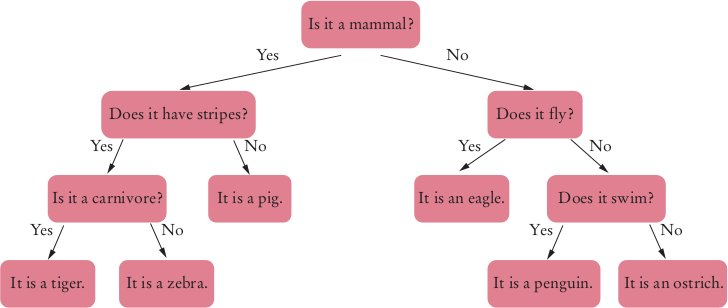
\includegraphics[width=0.8\linewidth]{decision-tree.jpg}
\caption{Пример дерева решений классификации животных}
\label{fig:decision-tree}
\end{figure}

В зависимости от решаемой задачи в листьях дерева могут храниться значение одного из двух основных типов: либо это конкретный класс рассматриваемой предметной области при решении задачи классификации, либо число (регрессионная модель), определяющее вероятность наступления некоторого события (победа команды в предстоящем матче) или прогнозируемую величину исследуемой функции (цена от продажи квартиры). В качестве входных данных дерево решений принимает массив параметров с опорной информацией, используемой в узлах дерева для определения перехода, например, для расчета вероятности выигрыша футбольной команды это будут: информация о положении в турнирной таблице, погоде и предыдущих играх.

\subsection{Общий подход формирования дерева}
\hspace{\parindent} Деревья решений имеют очень простую и наглядную структуру, что позволяет формировать их вручную для небольшого набора данных. Тем не менее, существуют разные схемы для автоматического обучения и выращивания деревьев. Каждый из таких методов имеет свои преимущества и недостатки, но один из подходов стал основой большинства других решений, поскольку оказался очень быстродействующим и простым в реализации. Этот алгоритм известен под названием рекурсивного секционирования~\cite{quinlan1990decision} и действует по принципу инкрементного построения дерева.

Процесс выращивания начинается с пустого дерева и полного набора данных. Первым этапом решается задача поиска приемлемой точки разбиения исходной выборки на подмножества. С точки зрения реализации алгоритма, применяемый способ выбора атрибута разделения не имеет значения. Таким образом создается первый узел в дереве, разбивающий набор данных на несколько подмножеств, после чего данный процесс выполняется повторно, применительно к каждому из подмножеств, для создания поддеревьев. Критерий прекращения выращивания дерева выбирается в зависимости от решаемой задачи.

Для создания узлов принятия решений необходимо установить какими должны быть критерии секционирования. Как правило, при выборе атрибутов разбиения применяется жадный алгоритм, предусматривающий выбор наилучшего из приемлимых атрибутов.

\subsection{Функция оценки}
\hspace{\parindent} Основная идея при рекурсивном построении дерева --- это создание <<хорошего>> разбиения для текущего узла. Чтобы оценить качество получаемых поддеревьев и выбрать среди возможных вариантов самое оптимальное, вводят специальную функцию оценки. 

Для конкретности, рассмотрим пример построения дерева принятия решений задачи классификации. На вход подается тестовая выборка $<x_i,b_i>$, где $x_i$ --- $i$-ый вектор параметров, соответствующий классу $b_i$. Определено множество предикатов $H$ и каждый не листовой элемент дерева связан с некоторым $h \in H$. 

На рисунке~\ref{fig:range-split} показан пример классификатора, разбивающего двумерное пространство точек на четыре части. Множество предикатов задано функциями вида $H=\{x_i > \alpha | \alpha \in \mathbb{R}\}$.

\begin{figure}[h]
\begin{minipage}[h]{0.49\linewidth}
\center{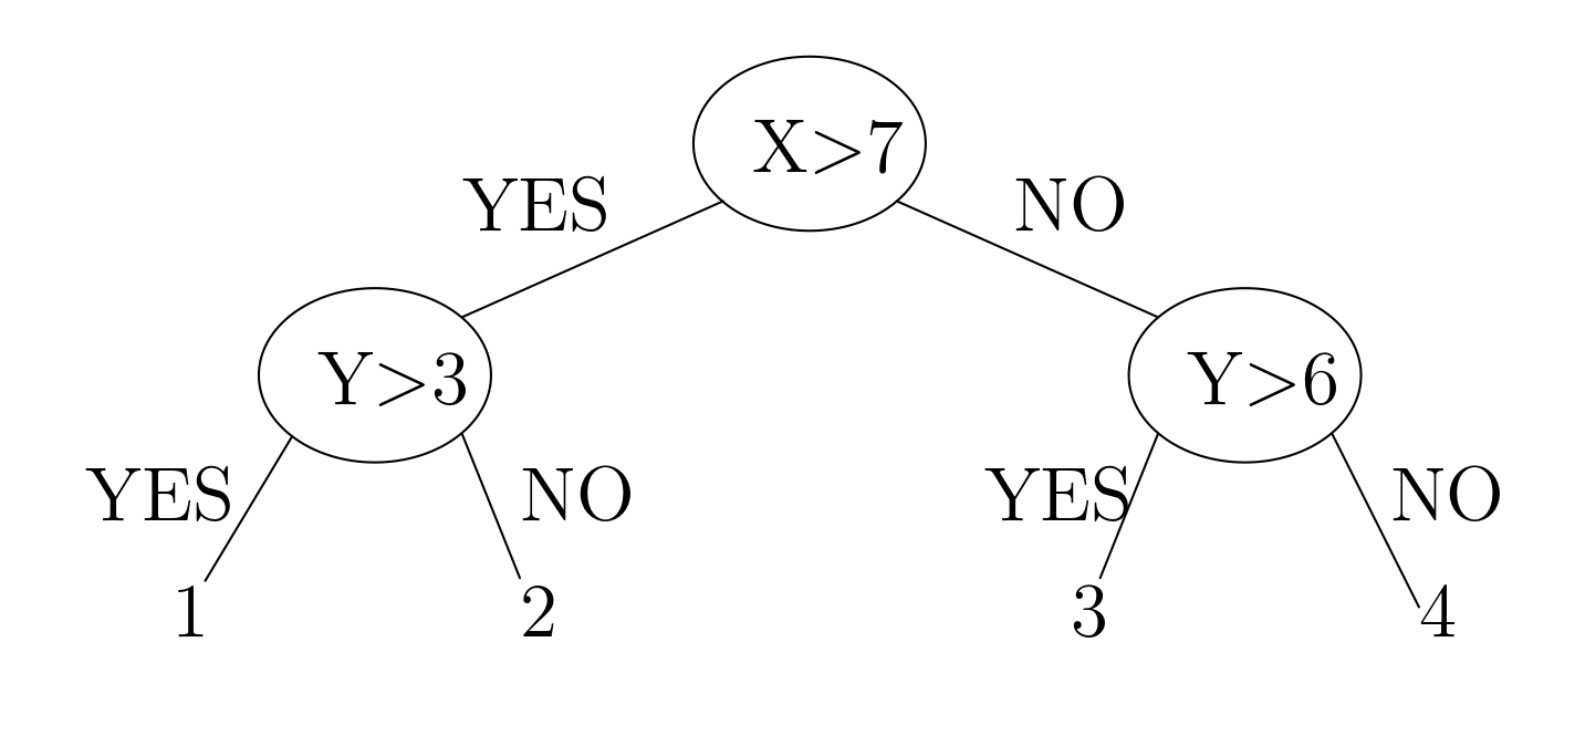
\includegraphics[width=0.8\linewidth]{tree-simple-predicat}}
\end{minipage}
\hfill
\begin{minipage}[h]{0.49\linewidth}
\center{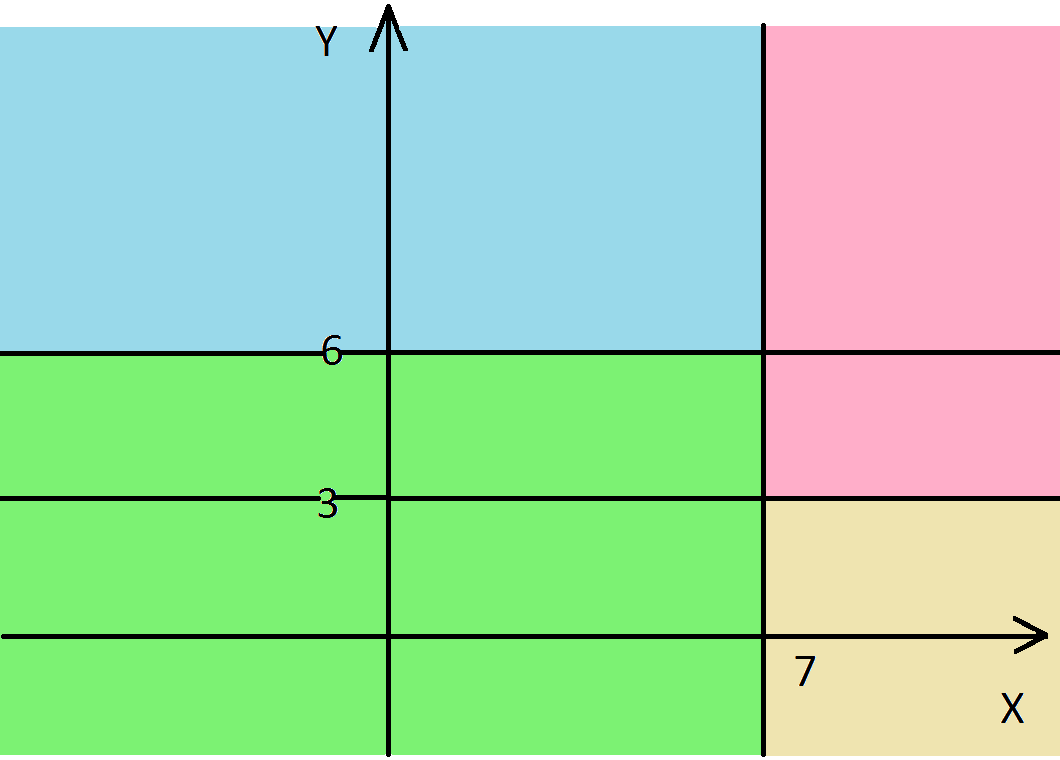
\includegraphics[width=0.7\linewidth]{split}}
\end{minipage}
\caption{Разбиение двумерного пространства точек деревом принятия решений; класс 1 --- розовый цвет, класс 2 --- желтый, класс 3 --- голубой и класс 4 --- зеленый}
\label{fig:range-split}
\end{figure}

Использование функции оценки при построении дерева должно увеличить точность создаваемого классификатора. Определим ошибку в каждой вершине $v$ как $E(v)$, следовательно суммарную ошибку по всему дереву можно вычислить как $E(T) = \sum\limits_{v \in T} Prob(v)E(v)$, где $T$ --- дерево принятия решений, а $Prob(v)$ --- вероятность перехода в вершину $v$, т. е. если по предикату $H$ из вершины $v$ осуществляется переход в одно из двух поддеревьев с корнями в вершинах $v_1$ и $v_2$, вероятности для них можно рассчитать по формулам:

$$
Prob(v_1) = P(H)
$$
$$
Prob(v_2) = 1 - P(H)
$$

\noindent где $P(H)$ --- вероятность перехода из вершины $v$ в $v_1$. На очередном этапе рекурсивного алгоритма выращивания в качестве функции оценки можно использовать $E(T)$, где $T$ --- это дерево с предполагаемым разбиением и корнем в текущей вершине. Однако, такой подход не всегда работает, например, если в исходной вершине $v$ наблюдалась ошибка $E(v)=0.2$ и один из вариантов ее разделения предполагает добавление двух новых вершин $v_1$ и $v_2$ с равновероятными переходами $P(H)=0.5$ и вероятностью ошибки $E(v_1)=0.4$ и $E(v_2)=0$, то итоговая ошибка $E(v)$ никак не изменится $E(v)=0.5*0.4+0.5*0=0.2$, хотя в результате такого разбиения одна из веток дает сто процентный результат классификации.

\subsection{Построение сверху-вниз}
\hspace{\parindent} Функцию $E(T)$ можно использовать для оценки качества уже построенного дерева, а не для выбора одного из множества поддеревьев на этапе разбиения. Таким образом, выращивая дерево, можно говорить о решении задачи минимизации функции $E(T_i)$, где $T_i$ --- множество всех возможных классификационных деревьев. 

Пусть для некоторого предиката $h \in H$, терм $T(l, h)$ определяет дерево, в котором у листа $l$ существует два новых дочерних элемента, переход в которые осуществляется по $h$. Тогда алгоритм построения можно определить следующим образом: на вход подается множество $H$ и максимальный размер дерева $t$, построение начинается с дерева $T_0$, состоящим из одной вершины, и далее по алгоритму

\begin{enumerate}
\item Закончить выращивание, если размер дерева больше установленного ограничения $t$
\item Построить новое дерево $T_{i+1} \leftarrow min_{l \in T, h \in H}(E(T_i)-E(T_i(l, h)))$
\end{enumerate}

По такому принципу работают алгоритмы CART и С4.5, названный в 2008 году алгоритмом машинного обучения №1~\cite{wu2008top}. Эти алгоритмы доступны в качестве готовых библиотек для языка программирования Python. С их помощью можно легко вырастить дерево для задачи классификации ирисов Фишера (рисунок~\ref{fig:Iris-Fisher}) --- набора данных, на примере которого Рональд Фишер в 1936 году продемонстрировал работу разработанного им метода дискриминантного анализа~\cite{fisher1936use}. 

\begin{figure}[h]
\begin{minipage}[h]{0.49\linewidth}
\center{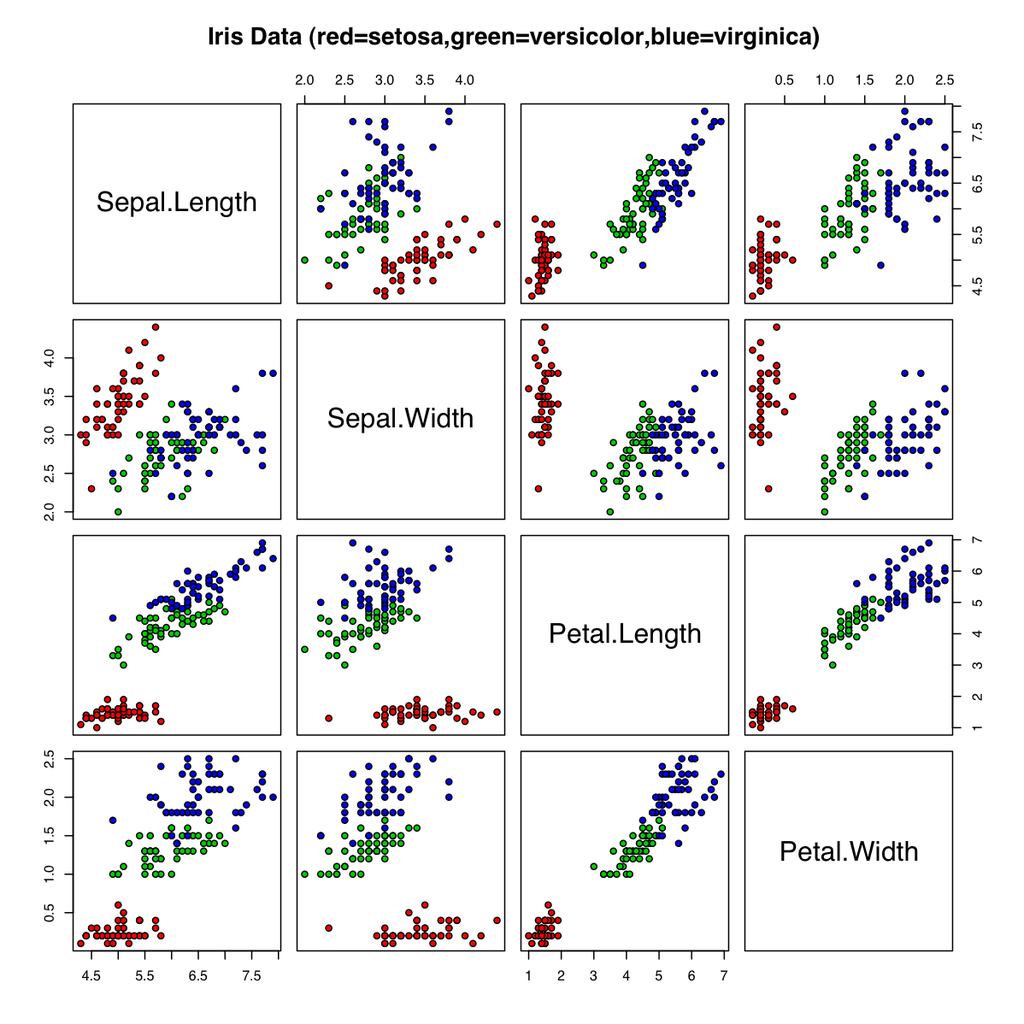
\includegraphics[width=1\linewidth]{FisherIris} \\ а) }
\end{minipage}
\hfill
\begin{minipage}[h]{0.49\linewidth}
\center{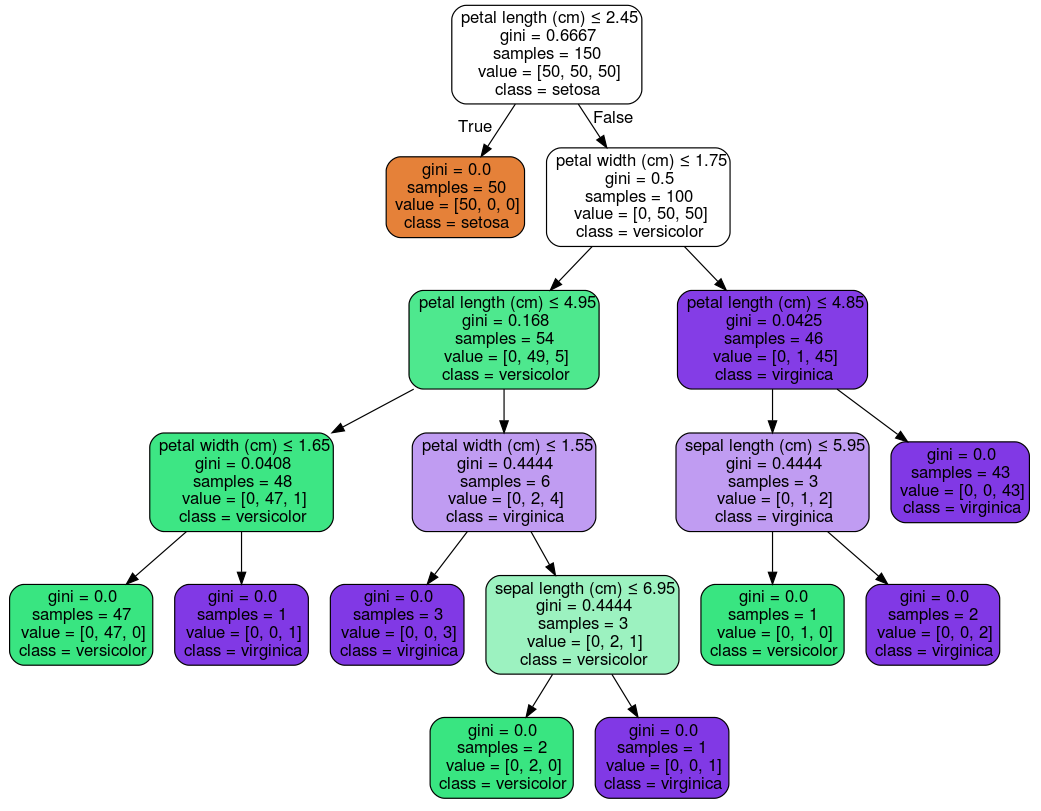
\includegraphics[width=1\linewidth]{iris-tree} \\ б)}
\end{minipage}
\caption{а) Диаграмма рассеяния ирисов Фишера \\ б) Дерево принятия решений для классификации ирисов Фишера}
\label{fig:Iris-Fisher}
\end{figure}

\subsection{Процедура обучения}
\hspace{\parindent} При использовании автоматических методов построения деревьев принятия решений отдельное внимание необходимо уделять обучающей выборке чтобы не допустить переобучения (overfitting) --- ситуации, когда во входном наборе данных обнаруживаются некоторые случайные закономерности, отсутствующие в генеральной совокупности. В противном случае, полученная модель является недостаточно общей.

Один из подходов борьбы с проблемой переобучения заключается в заготовке качественных наборов данных, разделенных на три группы:
\begin{itemize}
\item Обучающее множество, которое используется в алгоритме рекурсивного секционирования.
\item Аттестационное множество, для усовершенствования дерева решений, полученного в результате обучения.
\item Проверочное множество, позволяющее выполнить окончательную проверку результатов обучения для подтверждения применимости полученного дерева решений.
\end{itemize}

\subsection{Отсечение веток}
\hspace{\parindent} Отсечение частей дерева решений (pruning) является алгоритмом улучшения качества и осуществляется на этапе обработки, который следует за обучением. Для его работы необходимо иметь аттестационное множество, отличное от обучающей выборки. Метод основан на предположении, что в дереве существуют ребра, убрав которые произойдет увеличение точности.

Для того чтобы осуществить подобную проверку, необходимо знать, какое промежуточное значение накапливается в каждом узле принятия решений. Далее происходит тестирование дерева на всем аттестационном множестве с подсчетом успешно классифицированных наборов данных в каждой вершине. Если окажется, что некоторый узел имеет лучшую оценку, чем сумма всех его сыновей, то происходит усечение дерева (рисунок~\ref{fig:amputation}).

\begin{figure}[H]
\centering
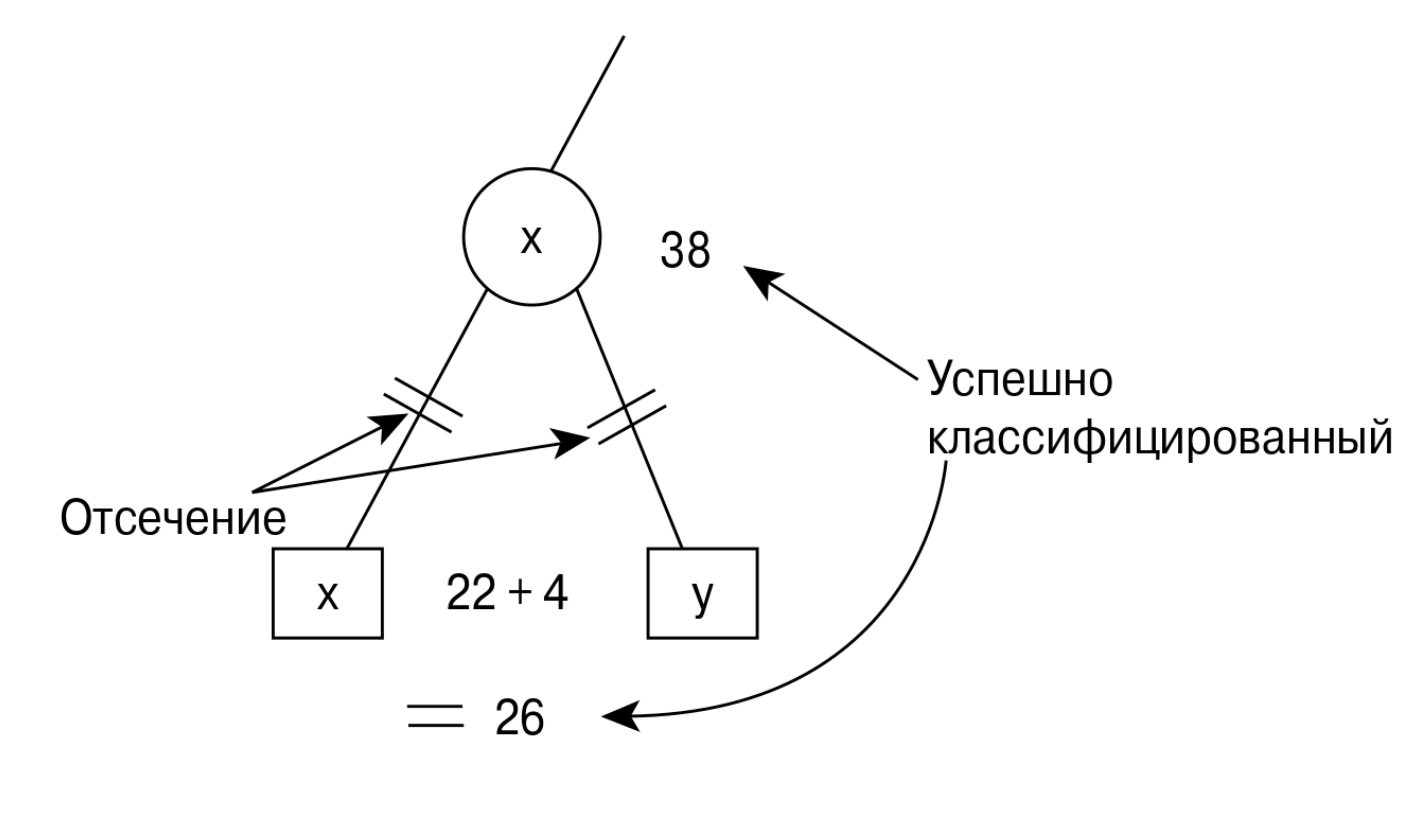
\includegraphics[width=0.85\linewidth]{amputation}
\caption{Отсечение ребер дерева после подсчета успешно классифицированных примеров}
\label{fig:amputation}
\end{figure}

\subsection{Случайный лес}
\hspace{\parindent} Метод случайного леса (random forest) основан на использовании комитета (ансамбля) деревьев принятия решений. Он был предложен Leo Breiman~\cite{breiman2001random}, одним из создателей алгоритма  для построения бинарного дерева решений (CART). Метод дает высокое качество результата, лучше чем у нейронных сетей~\cite{niculescu2005empirical}, эффективно обрабатывает данные с большим числом признаков классов, обладает возможностью оценивать значимости отдельных признаков в модели.

При обучении создается выборка из $N$ примеров, а также задаются размерность пространства признаков $M$ и дополнительный параметр $m$ (для задач классификации обычно выбирается $m \approx sqrt(M)$). Все деревья комитета строятся независимо друг от друга по следующей процедуре:
\begin{itemize}
\item Генерируется случайное подмножество с повторениями размером $N$ из множества обучающей выборки.
\item Выращивается решающее дерево, классифицирующее примеры данного подмножества, причём в ходе создания очередного узла выбирается признак не из всего пространства признаков размерности $M$, а лишь из $m$ случайно выбранных. 
\item Дерево строится до полного исчерпания подмножества примеров и не обрабатывается процедурами улучшения результата (такими как отсечение веток).
\end{itemize}

Классификация объектов проводится путём голосования: каждое дерево комитета относит классифицируемый объект к одному из классов, и побеждает тот, за который проголосовало наибольшее число деревьев. Размерность леса подбирается таким образом, чтобы минимизировать ошибку классификатора на тестовой выборке. 

Случайные леса могут быть естественным образом использованы для оценки важности переменных в задачах регрессии и классификации. Меняя параметры выборки, и определяя точки максимумов можно установить какие из них являются более важными для тренировочного набора. 

Использование случайного леса для задачи классификации изображений вместе с алгоритмами выделения регионов интереса (ROI --- Region Of Interest) дает хорошие результаты~\cite{bosch2007image}.

\newpage

\section{Нейронные сети}
\hspace{\parindent} Под нейронными сетями понимают математическую модель самообучающейся системы, имитирующей деятельность нервных клеток в биологических нейронных сетях. Понятие возникло при изучении процессов, протекающих в мозге, и при попытке их моделирования. Несмотря на большое разнообразие вариантов нейронных сетей, все они состоят из большого числа связанных между собой однотипных элементов --- нейронов, иммитирующих одноименные клетки живых организмов.

Искусственный нейрон, так же, как и живой, состоит из синапсов, связывающих его входы с ядром, которое осуществляет обработку входных сигналов. Связь с нейронами следующего слоя происходит через аксон. Каждый синапс имеет вес, определяющий насколько соответствующий вход нейрона влияет на его состояние, вычисляемое по формуле~\ref{eq:neuron-state}, 
\begin{equation}
S = \sum_{i=1}^{n}x_iw_i
\label{eq:neuron-state}
\end{equation} 

\noindent где $n$ --- число входов нейрона, $x_i$ --- значение $i$-го входа нейрона, $w_i$ --- вес $i$-го синапса. Значение аксона вычисляется как $f(S)$. Функция $f$ называется активационной и может быть своей у каждого нейрона сети. На рисунке~\ref{fig:Neuralnetwork} показан пример нейросети, состоящей из трех слоев: входные нейроны (зеленый цвет), скрытые (синий) и выходной нейрон (желтый).
\begin{figure}[H]
\centering
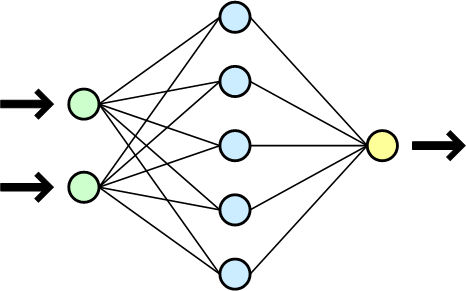
\includegraphics[width=0.7\linewidth]{Neuralnetwork}
\caption{Схема простой нейросети}
\label{fig:Neuralnetwork}
\end{figure}

Нейронные сети активно используются в задачах распознавания образов и предсказывания. Их часто применяют в области машинного обучения, называющейся глубокое обучение (deep learning), занимающейся моделированием высокоуровневых абстракций данных, используя системы со сложной архитектурой из множества нелинейных трансформаций. Под глубиной понимается максимальная длина между входным и выходным узлами графа вычислений модели.

\subsection{Нейронные сети обратного распространения}
\hspace{\parindent} Алгоритм обратного распространения ошибки (back propagation) является одним из методов обучения многослойных нейронных сетей прямого распространения, называемых также многослойными персептронами. Данный подход предполагает два прохода по всем слоям сети: прямой, при котором вычисляется реакция на заданный входной образ, и обратный, редактирующий синаптические веса с целью максимального приближения выходного сигнала сети к желаемому. 

Рассмотрим работу алгоритма на примере обучения нейронной сети, представленной на рисунке~\ref{fig:NN_multilayer_networks_01}.

\begin{figure}[h]
\centering
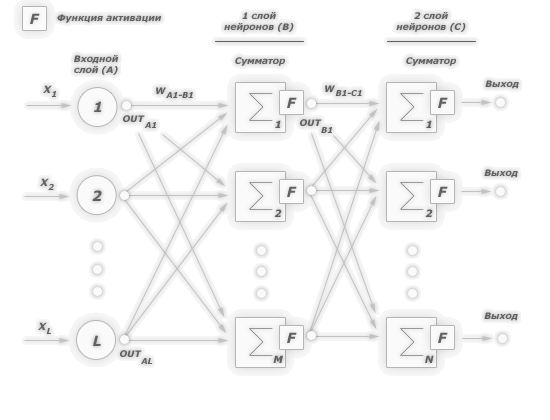
\includegraphics[width=0.75\linewidth]{NN_multilayer_networks_01}
\caption{Пример двухслойного персептрона}
\label{fig:NN_multilayer_networks_01}
\end{figure}

В качестве активационной, используется сигмоидальная логистическая функция (\ref{eq:sigmoid}), где $\alpha$ --- параметром наклона, изменяя который можно управлять крутизной графика. Сигмоид нормирует входной сигнал, возвращая значение из диапазона от нуля до единицы. Для алгоритма обратного распространения ошибки от активационной функции требуется только выполнения условия всюду дифференцируемости. Сигмоид удовлетворяет этому требованию, а его дополнительное преимущество состоит в автоматическом контроле усиления: для слабых сигналов кривая вход-выход имеет сильный наклон, дающий большое усиление, но когда величина сигнала становится больше, усиление падает. Таким образом, большие сигналы воспринимаются сетью без насыщения, а слабые проходят без чрезмерного ослабления. 

\begin{equation}\label{eq:sigmoid}
f(x)=\frac{1}{1+e^{-\alpha x}}
\end{equation}

Определим понятие обучающей пары --- это два вектора, один из которых задает входной сигнал для нейронной сети, а второй отвечает за требуемый выход. Обучение происходит на множестве обучающих пар, его целью является такая настройка синаптических весов, чтобы суммарное отклонение (функция ошибки) от желаемого результата было минимально. Ошибку нейронной сети для каждого теста обучающей выборки можно вычислить по методу наименьших квадратов (\ref{eq:kvadrat-error}),

\begin{equation}\label{eq:kvadrat-error}
E(w) = \frac{1}{2} \sum\limits_{i=1}^{p} (d_i-y_i)^2
\end{equation}

\noindent где $y_i$ --- значение $i$-го выхода нейросети, $d_i$ --- ожидаемое значение, $p$ --- число нейронов в выходном слое.

Таким образом, ставится задача многомерной минимизации, для решения которой используется метод градиентного спуска. На основании каждой обучающей пары происходит корректировка синаптических весов сети $w_{ij}$ на некоторое число~(\ref{eq:gradient-delta}),

\begin{equation}\label{eq:gradient-delta}
\Delta w_{ij}=-\eta \frac{\delta E}{\delta w_{ij}}
\end{equation}

\noindent где $0<\eta < 1$ --- множитель, задающий скорость движения вдоль направления аниградиента.

В рассматриваемом примере веса $w_{B_i-C_j}$ влияют на выход сети только как часть суммы $S_{C_j} = \sum w_{B_i-C_j} x_{C_j}$ по входам $j$-го узла, поэтому

$$
\frac{\delta E}{\delta w_{B_i-C_j}} = \frac{\delta E}{\delta S_{C_j}} \frac{\delta S_{C_j}}{\delta w_{B_i-C_j}} = x_{C_j} \frac{\delta E}{\delta S_{C_j}}
$$

Так как сейчас мы рассматриваем выходной слой сети $C$, следовательно, $S_{C_j}$ влияет на общую ошибку только в рамках выхода своего узла $C_j$:

\begin{eqnarray}\label{eq:out-layer-error}
\frac{\delta E}{\delta S_{C_j}} = \frac{\delta E}{\delta y_j} \frac{\delta y_j}{\delta  S_{C_j}} = \left(\frac{\delta}{\delta y_j} \frac{1}{2} \sum\limits_{i \in C} (d_i-y_i)^2\right)\left(\frac{\delta f(S_{C_j})}{\delta S_{C_j}}\right) = \nonumber \\ \left(\frac{1}{2}\frac{\delta}{\delta y_j}(d_j-y_j)^2\right)\left(y_j(1-y_j)\right)\alpha = -\alpha y_j(1-y_j)(d_j-y_j)
\end{eqnarray}

Введем обозначение $Children(X_j)$ определяющее множество выходов для $j$-го нейрона слоя $X$. Тогда для внутренних слоев сети, для конкретности рассмотрим $A$, получается:

$$
\frac{\delta E}{\delta S_{A_j}} = \sum_{k \in Children(A_j)} \frac{\delta E}{\delta S_k} \frac{\delta S_k}{\delta S_{A_j}} 
$$
\begin{eqnarray}\label{eq:in-layer}
\frac{\delta S_k}{\delta S_{A_j}}=\frac{\delta S_k}{\delta y_{A_j}} \frac{\delta y_{A_j}}{\delta S_{A_j}}=w_{A_j-B_k}\frac{\delta y_{A_j}}{\delta S_{A_j}}=\alpha w_{A_j-B_k} y_{A_j}(1-y_{A_j})
\end{eqnarray}

Таким образом, корректировка синаптических весов для выходного слоя нейронов происходит по формуле~(\ref{eq:out-layer-error}), а для внутренних (\ref{eq:in-layer}). Необходимо отметить, что простейший метод градиентного спуска, рассмотренный выше, неэффективен если производные по различным весам сильно отличаются. В этом случае для плавного уменьшения ошибки надо выбирать очень маленькую скорость обучения, но при этом существенно возрастает время работы алгоритма. Для выхода из этой ситуации можно применить метод введения момента, когда со временем происходит изменение влияния градиента на корректировку весов. Такой подход также используется для выхода из точек локального минимума.

\subsection{Задача распознавания изображений}
\hspace{\parindent} Рассмотрим задачу распознавания рукописных цифр. Необходимо создать и обучить нейросеть, которая по заданному изображению активирует один из дести выходов. В качестве входных данных рассматривается база рукописных цифр MNIST~\cite{lecun1998mnist}, содержащая шестьдесят тысяч обучающих пар (изображение --- метка) и десяти тысяч тестовых (изображения без меток). Картинки нормализованы по размеру и отцентрованы. Размер каждой цифры не более $20\times20$ пикселей, и все они вписаны в квадрат размером $28\times28$. Пример первой дюжины цифр из обучающего набора базы MNIST приведен на рисунке~\ref{fig:mnist}.

\begin{figure}[h]
\centering
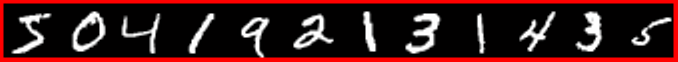
\includegraphics[width=0.7\linewidth]{mnist}
\caption{Пример цифр из обучающего набора базы MNIST}
\label{fig:mnist}
\end{figure}

При использовании нейронных сетей для решения этой задачи возникает ряд вопросов, связанных с тем как подать данные в сеть и какую архитектуру (количество скрытых слоев, уровень связности) использовать. На текущий момент до сих пор не существует методов, позволяющих однозначно определить структуру и состав нейросети исходя из описания задачи. Есть множество различных методик редукции (например OBD~\cite{chauvin1989advances}), а также разные эвристики и эмпирические правила, одно из которых гласит, что количество нейронов в скрытом слое должно быть хотя бы на порядок больше количества входов.

Один из подходов загрузки изображения в нейросеть заключается в представлении двумерной матрицы исходной картинки в виде одномерного вектора. Согласно описанной выше эвристике и использовании полносвязной нейронной сети получается что итоговая модель будет иметь $\prod_{i=1}^{N} len(X_i)\times len(X_{i+1})$ связей, где $N$ --- количество слоев, а $len(X)$ --- размер слоя $X$. Таким образом, для рассматриваемой задачи распознавания рукописной цифры получается $28\times28=784$ нейрона на входном слое, а при использовании двух слоев по десять и пять тысяч нейронов в каждом, около шестидесяти миллионов связей (десять миллионов между входным и первым скрытым слоем, пятьдесят миллионов между первым и вторым и пятьдесят тысяч между вторым и выходным).

При преобразовании изображения в линейную цепочку байт, происходит потеря взаимосвязи между отдельными частями входной картинки, а решаемая задача распознавания подразумевает умение нейросети быть устойчивой к небольшим сдвигам, поворотам и изменению масштаба изображения, а значит она должна извлекать из данных некие инварианты, не зависящие от почерка того или иного человека. Таким образом, полносвязные нейронные сети обратного распространения не очень хорошо подходят для распознавания образов, так как являются очень вычислительно сложным решением и, в тоже время, не способны корректно справляться с различными искажениями входных изображений.

\subsection{Сверточные нейронные сети}
\hspace{\parindent} Сверточная нейронная сеть (CNN --- Convolutional Neural Network) --- это специальная архитектура искусственных нейронных сетей, нацеленная на эффективное распознавание изображений и предложенная Яном Лекуном~\cite{lecuncomparison}, вдохновленным работами нобелевских лауреатов в области медицины Torsten Nils Wiesel и David H. Hubel. Эти ученые исследовали зрительную кору головного мозга кошки и обнаружили, что существуют так называемые простые клетки, которые особо сильно реагируют на прямые линии под разными углами и сложные клетки, которые реагирую на движение линий в одном направлении. 

Идея архитектуры сети заключается в чередовании сверточных слоев (C-layers), субдискретизирующих слоев (S-layers) и наличии полносвязных (F-layers) слоев на выходе, структура --- однонаправленная (без обратных связей). В качестве активационной используется любая функция по выбору исследователя. Название архитектура сети получила из-за наличия операции свёртки, суть которой в том, что каждый фрагмент изображения умножается на матрицу (ядро) свёртки поэлементно, а результат суммируется и записывается в аналогичную позицию выходного изображения.

При данном подходе рассматриваются три основные парадигмы:
\begin{itemize}
\item Локальное восприятие
\item Разделяемые веса
\item Субдискретизация
\end{itemize}

\newpage
\section*{Используемые обозначения}
ANN --- Artificial Neural Network, искуственная нейронная сеть (тоже самое что и NN)

\noindent Back propagation --- алгоритм обратного распространения ошибки обучения многослойных нейронных сетей 

\noindent CART --- Classification And Regression Trees, алгоритм  для построения бинарного дерева решений

\noindent CNN --- Convolutional Neural Network, сверточная нейронная сеть

\noindent Data mining --- автоматические методы интеллектуального анализа

\noindent Decision tree --- деревья принятия решений

\noindent Deep learning --- область машинного обучения, занимающаяся моделированием высокоуровневых абстракций данных, используя системы со сложной архитектурой из множества нелинейных трансформаций

\noindent Fine tuning --- алгоритмы частичной корректировки коэффициентов модели при ее дообучении

\noindent Information extraction --- методы автоматического выделения информации

\noindent Logistic function --- сигмоидальная функция 

\noindent Logistic neuron --- нейрон с сигмоидальной активационной функцией

\noindent ML --- Machine Learning, машинное обучение

\noindent NN --- Neural Network, нейронная сеть

\noindent MNIST --- база данных рукописных цифр

\noindent Pruning --- отсечение веток дерева решений, алгоритм улучшения качества

\noindent OBD --- Optimal Brain Damage, метод редукции нейросети

\noindent OCR --- Optical Character Recognition, задача распознавания рукописного текста

\noindent Overfitting --- переобучение 

\noindent Random forest --- комитета решающих деревьев для задач классификации и регрессии

\noindent ROI --- Region Of Interest 

\newpage
\bibliographystyle{gost780u}  %% стилевой файл для оформления по ГОСТу
\begin{flushleft}
\bibliography{biblio}     %% имя библиографической базы (bib-файла) 
\end{flushleft}

\end{document}